% !TEX TS-program = pdflatex
% !TEX encoding = UTF-8 Unicode

% This is a simple template for a LaTeX document using the "article" class.
% See "book", "report", "letter" for other types of document.

\documentclass[12pt]{article} % use larger type; default would be 10pt


\usepackage[utf8]{inputenc} % set input encoding (not needed with XeLaTeX)

%%% Examples of Article customizations
% These packages are optional, depending whether you want the features they provide.
% See the LaTeX Companion or other references for full information.

%%% PAGE DIMENSIONS
\usepackage{geometry} % to change the page dimensions
\geometry{a4paper} % or letterpaper (US) or a5paper or....
% \geometry{margin=2in} % for example, change the margins to 2 inches all round
% \geometry{landscape} % set up the page for landscape
%   read geometry.pdf for detailed page layout information

\linespread{1.5}

\usepackage{graphicx} % support the \includegraphics command and options
\usepackage{float}
% \usepackage[parfill]{parskip} % Activate to begin paragraphs with an empty line rather than an indent

%%% PACKAGES
\usepackage[ comma, sort&compress]{natbib}
\usepackage{booktabs} % for much better looking tables
\usepackage{array} % for better arrays (eg matrices) in maths
\usepackage{paralist} % very flexible & customisable lists (eg. enumerate/itemize, etc.)
\usepackage{verbatim} % adds environment for commenting out blocks of text & for better verbatim
\usepackage{amsmath}
\usepackage{subfig} % make it possible to include more than one captioned figure/table in a single float
% These packages are all incorporated in the memoir class to one degree or another...
\usepackage{bm}

%%% HEADERS & FOOTERS
\usepackage{fancyhdr} % This should be set AFTER setting up the page geometry
\pagestyle{fancy} % options: empty , plain , fancy
\renewcommand{\headrulewidth}{0pt} % customise the layout...
\lhead{}\chead{}\rhead{}
\lfoot{}\cfoot{\thepage}\rfoot{}

%%% SECTION TITLE APPEARANCE
\usepackage{sectsty}
\allsectionsfont{\bfseries\upshape} % (See the fntguide.pdf for font help)
% (This matches ConTeXt defaults)

%%% ToC (table of contents) APPEARANCE
\usepackage[nottoc,notlof,notlot]{tocbibind} % Put the bibliography in the ToC
\usepackage[titles,subfigure]{tocloft} % Alter the style of the Table of Contents
\renewcommand{\cftsecfont}{\rmfamily\mdseries\upshape}
\renewcommand{\cftsecpagefont}{\rmfamily\mdseries\upshape} % No bold!

%%% END Article customizations

%\date{}							% Activate to display a given date or no date

\begin{document}

\title{ECON 706 - Problem Set 2}
\author{Andr\'e Victor D. Luduvice, Stefano Pietrosanti and Joseph Silverstein}

\maketitle

\begin{abstract}
In this problem set we study the behavior of housing completions and starts in the frequency domain. We conduct detailed spectral analysis of the series both for univariate and multivariate cases, both with parametric and nonparametric techniques, so to investigate the underling cyclical behavior of housing starts and completions. 

\end{abstract}

\section{Introduction}

With the present work, we extend on the time domain analysis of Problem Set 1, so to consider the frequency domain behavior of the time series under study. We again work on the FED of St. Louis data set, \citep{dataset}, collecting the US Census's results.

The time series under study collect 45 years plus one month of monthly observation of housing starts and completions, from January 1970 to January 2015, for a total of 541 observations.

The article is organized in two sections: Univariate and Multivariate Analysis; these sections are then subdivided on the basis of the methods employed (lag-window, autoregressive, etc...), and methods are grouped with respect to whether they are parametric, or non-parametric.

\subsection{Methodology}

One of the most important aspects of Spectral Analysis is to analyze the variability of a stochastic processes over the frequencies rather than over the time domain. This means to look at the Periodgram instead that investigating the Autocorrelation. Thus changing perspective, we try to observe the Time$\;\times\;$Level space as filled by many possible wave (sine-cosine) functions, each for a different frequency.

E.g., we can take a cosine function, and think to have a finite series of length $T$ - this only for the present paragraph, for clarity sake. The $cos(u)$ function is defined over the $[0,2\pi]$ space (actually, it is defined over $[-\pi,\pi]$, but being symmetric we can lightheartedly shift to the positive radiants). Let see the $u$ unit over the circle in the following way: $u(\omega, t)=2\pi*\frac{k}{T}*t$, where $T$ is the total of our time observations; $t$ is specific time point; $k$ the number of cycles our wave completes in the time span we observe; hence, $\omega_k=\frac{2\pi*k}{T}$.  We have thus restated the wave function on the Time-Value space, where the measure $2\pi$ over the circle is mapped (if possible) to the $t=\frac{T}{k}$ data point, and so on and so forth\footnote{
Hence moving to an infinite sample makes what above imprecise, yet not the intuition. With an infinite sample we can in principle observe an infinite number of cycles.}.

As we do this, we consider (loosely following \citet{hammy}, as in all other comments) data points as $x_t$, from the generic stationary time series $\{x_t\}_t$, as the result of the composition of these different sine and cosine waves at different frequencies. 

\begin{equation}
\begin{aligned}
x_t=\sum_k(a_k*\text{sin}(\omega_k*t)+b_k*\text{cos}(\omega_k*t))
\end{aligned}
\end{equation}

We can recognize something similar to a linear regression.
With ``similar'', we mean that we can estimate this as an actual linear regression with perfect fit (why perfect fit is explained in the footnote n.1), considering $a_k\,,\,b_k$ as coefficients. Yet, as long as we stay on theoretical ground, we must state that these coefficients are zero mean, equal variance ($\sigma_k^2$), serially and mutually uncorrelated random variables. As in the regression framework, some $k$ indexed explanatories will be more important and other less\footnote{
When working with an actual sample of $T$ observations, the maximum possible $k$ is $\frac{T}{2}$. This since, with $T$ observation, we can have at most $T$ explanatories; each $k$ brings with itself a sine and a cosine explanatory both, hence we can at most have $T$ over a half $k$s, and perfect fit. Since we want to check for the contribution of all possible frequencies, we sum over $k\in\left\{0,\frac{T}{2}\right\}$, and we go for the perfect fit.}. To measure this ``importance'', we can ask ourselves the classical ANOVA question: ``how much this component helps explaining the total variability?". To answer such question we can observe that\footnote{We assume that $x_t$ is mean zero.}

\begin{equation}
\begin{aligned}
E[x_t^2]=\gamma(0)=\sum_k(E[a_k^2]*\text{sin}(\omega_k*t)^2+E[b_k^2]*\text{cos}(\omega_k*t)^2)=\\
=\sum_k\,\sigma_k^2
\end{aligned}
\end{equation}

We also know that the $\gamma(0)$ is just one instance of the autocovariance function, which we can recast completely on the frequency domain using the autocovariance generating function. For each frequency $\omega$ we have:

\begin{equation}
\begin{aligned}
g_X=\sum\limits_{t=-\infty}^{\infty} \gamma(t)z^t \\
\text{evaluate over the circle, hence}\; z=e^{-i\omega}\\
\text{and rescaling w.r.t.}\; 2\pi \;\text{we get}
s_X(\omega)=\sum\limits_{t=-\infty}^{\infty} \frac{1}{2\pi} \gamma(t)e^{-i\omega t}=\\
=\frac{1}{2\pi}\left[\gamma(0)+2\sum\limits_{t=-\infty}^{\infty} \gamma(t)\text{cos}(\omega t)\right]
\end{aligned}
\end{equation}

Where the last passage follows from the basic trigonometric identities and from symmetry of the involved functions around zero.
This last function is the population spectrum, a continuous, real valued function of the continuous frequency variable. Given that the Fourier transformation can be inverted, from the population spectrum we can recover frequencies as follows:

\begin{equation}
\begin{aligned}
\int_{-\pi}^{\pi} s_x(\omega)e^{-i\omega t}d\omega=\gamma(t)
\end{aligned}
\end{equation}

and the fact that the autocovariance of our stationary process is the integral of the spectrum over the frequencies for $t=0$ follows. We can appreciate how this works perfectly fine as long as we have infinitely many autocovariances. In a sample, with $T-1$ proper (not at lag 0) autocovariances, we will need to be careful. What follows is the tale of this carefulness. 

\newpage

\section{Univariate Analysis}

Here we are only interested in the study of the individual cyclical behavior of our series. A first and rough approach is to simply plot the raw Periodgram of our series. Though this estimator is unbiased, it is ridden with problems: first, a very large confidence interval that does not shrink with the increase in the number of data points considered (no consistency). We can think about this in the sine/cosine regression framework we stated in the introduction: as soon as we add new data to our sample, we can investigate new frequencies, hence we must add explanatories to our perfectly fit regressions.  The result is that - as the sample increases - we do not collect more information about the same parameters, but we add parameters instead.

The second problem is that, observing a cluster of peaks in the sample raw spectrum we are not totally sure about the ``importance ranking'' of the frequencies which correspond to these peaks. The main source of such a problem is the fact that the shift to frequency domain from time domain is a shift to a continuous space from a discrete space. As long as we have infinitely many discrete data points this is fine, and can be performed through Fourier transformation\footnote{As it is made clear in the Methodology section, where we see that the Fourier transform takes the lags of the autcovariances from $-\infty$ to $+\infty$.}. If we have finitely many discrete data points, though, we must take into account a lot of imprecision. This since, of the whole frequency line, we will only be able to consider the finitely many points spanned by $t$: $\frac{2\pi k}{T}t\;,\;t\in\left\{0,....,T\right\}$. Formally, the raw estimate is:

\begin{equation}
\begin{aligned}
\hat{s}_x(\omega)=\sum\limits_{t=-T+1}^{T-1} \frac{1}{2\pi} \gamma(t)e^{-i\omega t}=\\
=\frac{1}{2\pi}\left[\gamma(0)+2\sum\limits_{t=1}^{T-1} \gamma(t)\text{cos}(\omega t)\right]
\end{aligned}
\end{equation}

The underlying difficulty becomes clear as soon as we think to the theoretical Periodgram, which summarizes how frequency {\em till} a certain $\omega$ {\em continuously} contribute to the variance of the process. This contribution is described by the area encompassed by the {\em continuous} spectral density curve. If we try to estimate this with finitely many data points for each frequency {\em range}, we are estimating areas through points. Hence we are bound to see point contributions where actually contributions by {\em ranges} of frequencies are involved.

The result is pretty spiky and irregular (high - and irreducible - variance). Since this estimation is unbiased, though, it is a useful instrument to identify important ranges of frequencies, so to provide a ``reality check'' for our more sophisticated, consistent, yet often biased, estimation methods. 

Before showing the plots, a brief preliminary account about how we think about it. On the ordinate axis, we show the values of the estimated spectral densities, which - as for every density function - are arbitrary, such that the only relevant information conveyed is the relative magnitude. We look for peaks, for relatively high-weight (density) frequencies, since we are interested in the frequencies which are the most important for variance decomposition. On the abscissae axis, we instead plot the ``frequencies''. 

Yet here comes the tricky point, justifying our usage of quotes the last time we introduced the word frequencies. Since we employed the R's ``ts'' command to exploit the time series packages, it is as if we have been telling R to read frequencies over time, and not over the circle: an instance of the problem we mentioned before: for each frequency, we only have finitely many data points in the ${t}$ spanned world. 

Furthermore, also the number of cycles our waves can perform, $k$,  is constrained. Given that we are dealing with monthly observations, $T$ is the total number of monthly points constituting our series. Hence, the maximal number of cycles our explanatory wave functions can accomplish, over the $T=541$ periods we take into account, is $\frac{540}{2}$\footnote{Since we cannot show ``half-data ponts'', we solve the problem removing one observation, as in \citet{hammy}.}. This is a bimonthly frequency: the fastest wave we can consider completes six cycles each year. 

Consequently, setting 
\begin{verbatim}
freq=12
\end{verbatim} 
in the ``ts'' command, the Periodgram of any time series in our analysis will show frequency 6 as maximum abscissa. This means that the maximum number of cycles per year a wave component can complete in the environment of our analysis is 6.
This said, the plots follow:

\begin{figure}[H]
\begin{center}
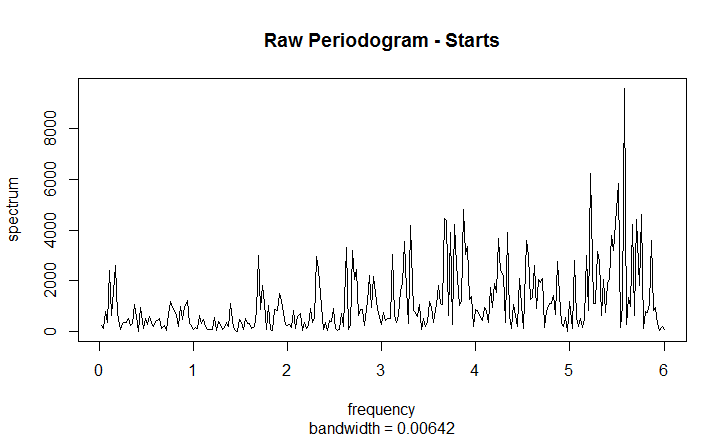
\includegraphics[scale=0.55]{rawspecstart}
\caption{}
\end{center}
\end{figure}

\begin{figure}[H]
\begin{center}
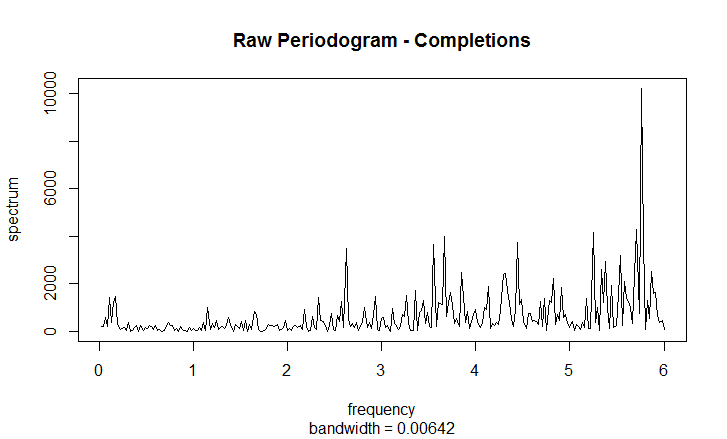
\includegraphics[scale=0.55]{rawspeccomp}
\caption{}
\end{center}
\end{figure}

As we can see, our series spectra are mostly coherent in shape, showing:

\begin{enumerate}
\item A low frequency component, which almost does not cycle, and hence has frequency concentrated near zero.
\item A group of spikes, located within the bi-quarterly and quarterly zone.
\item A very relevant (approximately) bi-monthly component, from which the most of the variability seems to be caused.
\end{enumerate}

Now we procede improving our estimates through Non-Parametric and Parametric methods.

\subsection{Non-Parametric}

Since the two main problems with the raw Periodgram are the improper concentration of spectral weight on single frequency points, and the inconsistent nature of the raw Periodgram as an estimator, it would be nice to have a solution for both. Fortunately this solution is there, is unique, and addresses both problems. In plain words, only looking at the estimate we previously got (non-parametric), we will try to smooth them in a ``clever'' way, so to diminish the variance (redistribute the concentrated weight) and get back consistency doing the smoothing over fixed intervals, so that the increase in the number of data will give us again more informations about what we are estimating.

Formally, $j$ being $\frac{k}{T}$, we use a $K(\omega_{j+m},\omega_j)$ (the {\em kernel}) weighting function\footnote{
In the sense that for each $h$, $\sum_{m=-h}^{h}K(\omega_{j+m},\omega_j)=1$.}, and we compute the estimates of the Periodgram on the base of the raw estimates:

\begin{equation}
\hat{s}_X=\sum\limits_{m=-h}^{h} K(\omega_{j+m},\omega_j)\hat{s}_x(\omega_j)
\end{equation}

where the $h$ is the bandwidth, i.e. how many raw correlation data points we exploit to estimate each element of our final approximation of the Periodgram\footnote{In the empirical analysis we define the bandwidth slightly differently: as $\frac{2h+1}{T}$, the total portion of disposable points we use for each estimate.}. This mitigate our two main problems. On the one hand, the fixed nature of the bandwidth allows us to regain consistency: as we increase the number of data points, more of them will fall into the bandwidth, so we go back to a world in which more data means more information; on the other hand, redistributing the weights, we curb the wild behavior of the raw Periodgram, so to better grasp the contribution of {\em ranges} of frequencies to the variance. On the other end, this procedure is biased by nature: if we smooth a previously unbiased estimate, and then we take again the average of the smoothed values, the result will be different from the previous average (which was unbiased). Hence we have a bias-variance trade off
 
\subsubsection{Spectral Window}

Since we only have the  $j=\frac{k}{T}$ frequencies at our disposal, in deciding the bandwidth we are deciding how many of these actually enter our smoothing procedure. This reasoning is at the base of the Spectral Window estimation method, in particular, we employ the modified Daniell's kernel. 

This last is simply a centered moving average, where the weight of the last two elements has been decreased in favor of the central elements (we are doing this to avoid the leakage of variance from one frequency range to the other). To let the weight concentrate on the very central value - and decrease linearly outside - we can apply the kernel multiple times (convoluting the kernel). In such case, the bandwidth of the resulting kernel (the convolution of the kernels considered as a single kernel) will be $\frac{n*h+1}{T}$\footnote{
Indeed, since in our final choice we opt for a two step convolution of the kernel, we have a bandwidth of $\frac{4*h+1}{T}$.}.

To do an actual example, let say we want the Spectral Window estimate of the Population Spectrum at the frequency $\omega_j$, $\hat{s}_X{\omega_j}$, we have the raw Periodgram estimate $\hat{s}_x{\omega_i}$ for $i\in\left\{0,...,\frac{T-1}{2}\right\}$; and we choose a bandwidth parameter equal to 1, applying it twice. This translates in the following mathematics:

\begin{equation}
\begin{aligned}
\hat{s}_X(\omega_j)_1=\frac{\hat{s}_x(\omega_{j-1})+\hat{s}_x(\omega_j)+\hat{s}_x(\omega_{j+1})}{3}\\
\text{then we apply the same kernel again, and we get}\\
\hat{s}_X(\omega_j)_2=\frac{\hat{s}_x(\omega_{j-2})+\hat{s}_x(\omega_{j+2})}{9}+\frac{2(\hat{s}_x(\omega_{j-1})+\hat{s}_x(\omega_{j+1}))}{9}+\frac{\hat{s}_x(\omega_j)}{3}
\end{aligned}
\end{equation}

The objective in this is to find the ``best'' way to smooth, hence the best bandwidth parameter. We do this {\em via} sheer comparison of the result of the application of different bandwidth parameters for both the applications of the kernel\footnote{
We can apply, say, $h=6$ the first time and $h=3$ the second time. Actually, we choose for $8,8$ for Start and $7,7$ for completions.}.

To do this we cycle through the bandwidth parameters for both the passages of the kernel. The nested loop computes the estimate for each couple of bandwidth parameters, and plot it along with the parametric estimate (to be commented later) and the raw estimate. 

I below show two extreme choices and the actual result for the Starts series(first the two extremes, then the result).

\begin{figure}[H]
\begin{center}
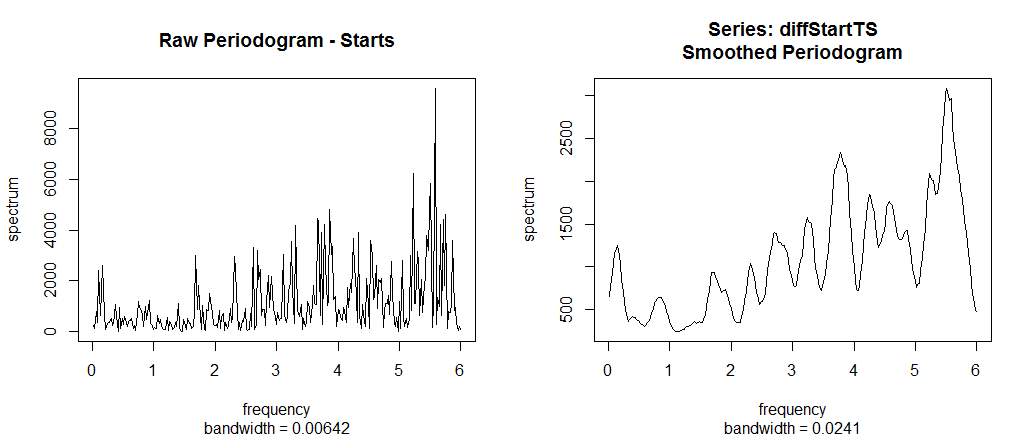
\includegraphics[scale=0.4]{spec33}
\caption{}
\end{center}
\end{figure}

\begin{figure}[H]
\begin{center}
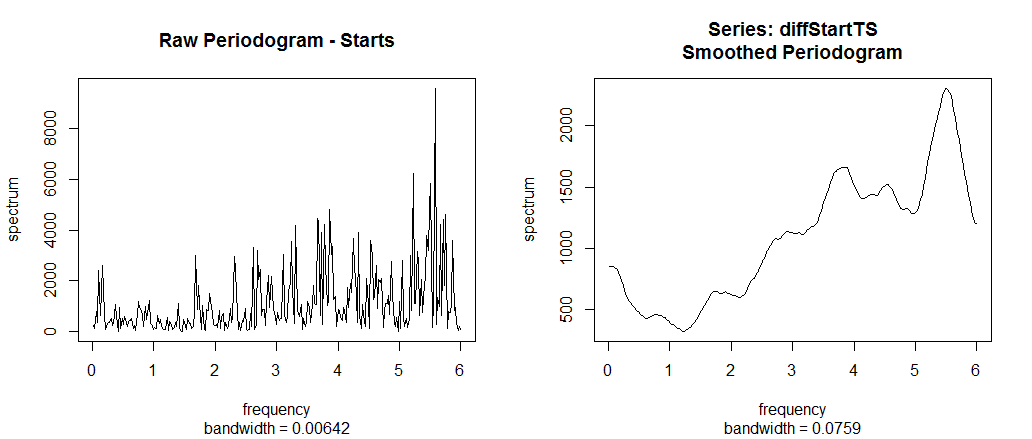
\includegraphics[scale=0.4]{spec1010}
\caption{}
\end{center}
\end{figure}

\begin{figure}[H]
\begin{center}
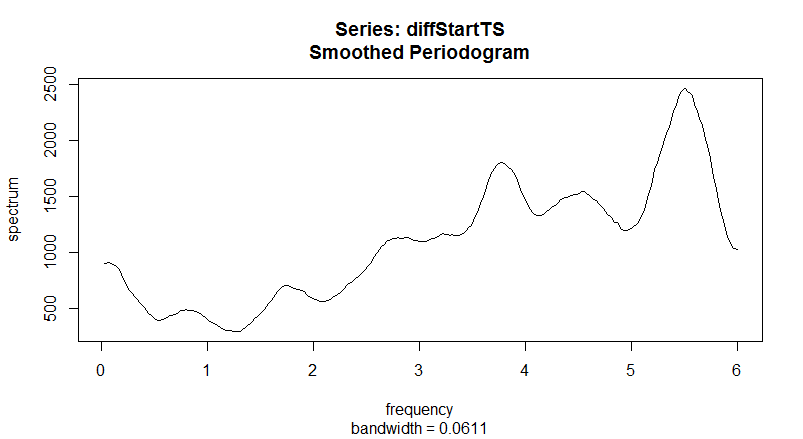
\includegraphics[scale=0.4]{spec88}
\caption{}
\end{center}
\end{figure}

As we can see, the graph for bandwidth $\frac{4*3+1}{540}=0.0241$ (lowest bandwidth considered for two passages) does not perform properly in its smoothing task. On the other hand, the $\frac{4*10+1}{540}=0.0759$ (looking at the raw estimation) is clearly biased, since it is over-smoothed, which results in a possible misestimation of the autocovariance of the sample at lag 0. Finally, the $\frac{4*8+1}{540}=0.0611$ accomplish the smoothing purpose without exceeding in it. So we settle on this choice.

The Completion final result follow, where the selection logic is the same.
 
\begin{figure}[H]
\begin{center}
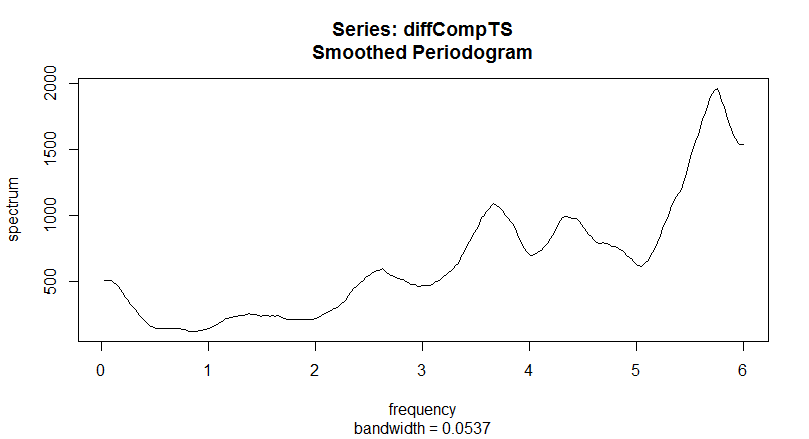
\includegraphics[scale=0.5]{spec77}
\caption{}
\end{center}
\end{figure}

\subsubsection{Lag Window}

The Lag Window differs from the Spectral Window with respect to the intuition and the type of kernel involved, yet the result is not this remarkably different - as we shall see.

First, the intuition. The main choice we had to perform with respect to the Spectral Window estimator was about over how many raw Periodgram point estimates we were going to smooth. Which is, over how many frequencies on the abscissae. 

For the Lag Window, we approach the issue from the autocorrelation perspective, for each frequency. We use the Bartlett kernel, defined as

\begin{equation}
\begin{aligned}
\kappa_j^*= \begin{cases}
      \text{if $t\in\left\{1,...,q\right\}$} &:\  
        1-\frac{t}{q+1}\\
      \text{otherwise} &:\ 0  
   \end{cases}
\end{aligned}
\end{equation}

We apply it, in combination with the sample autocovariances, in the following way:

\begin{equation}
\begin{aligned}
\hat{s}_X(\omega)=\frac{1}{2\pi}\left[\hat{\gamma}(0)+2\sum\limits_{t=1}^{q}\left( 1-\frac{t}{q+1}\right) \hat{\gamma}(t)\text{cos}(\omega t)\right]
\end{aligned}
\end{equation}

So, choosing $q$, we choose how many sample autocovariances to use in our estimation, as if there was some underlying, finite MA process involved. After a similar inspection procedure as the one employed for the Spectral window, we conclude that the best $q$ equals $25$ for the Starts series and $30$ for the Completion series. Given the closeness in the selection procedure with respect to the previous section, we will just show the final result 

Below the plots:

\begin{figure}[H]
\begin{center}
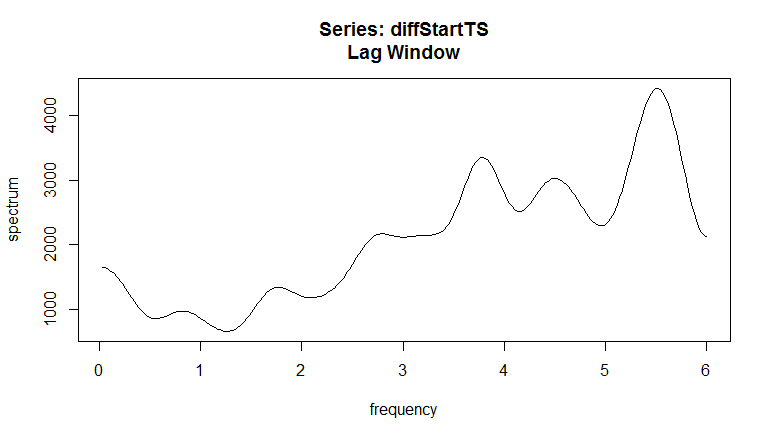
\includegraphics[scale=0.5]{lagstart}
\caption{}
\end{center}
\end{figure}

\begin{figure}[H]
\begin{center}
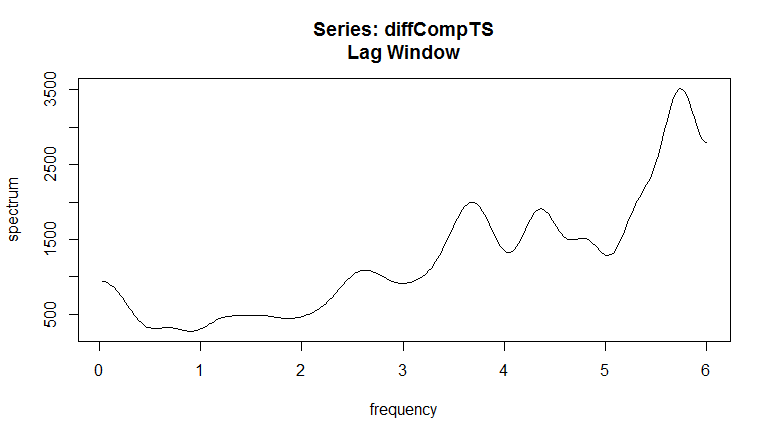
\includegraphics[scale=0.5]{lagcomp}
\caption{}
\end{center}
\end{figure}


\subsection{Parametric - Autoregressive Spectral Density Estimation}

A possible way to solve our estimation problem, given the close relationship between spectral density and variance of a stochastic process, is to exploit its underlying autoregressive structure to recover the spectral density. 

This procedure's underlying logic is\footnote{In the following I am using capital letters for the population, and non-labelled variables (as $\sigma$, the error's std deviation) for error related quantities.}: 

let assume we do know our generating process has a stationary, $\text{MA}(\infty)$ nature\footnote{
And we do: the time domain analysis showed how and $\text{ARIMA}(1,1,2)$ was a good approximation of both of the time series, so we have good evidence in favor of an $\text{MA}(\infty)$ of some sort generating the series of the {\em differences} in houses starts and completions.}. Then we know about the existence of an appropriate $\psi(\text{L})$ polynomial that describes this $\text{MA}(\infty)$ process, which means we can refer to the following autocovariance generating function:

\begin{equation}
\begin{aligned}
g_X(z)=\sigma^2\psi(z)\psi(z^-1)
\end{aligned}
\end{equation}

We can then evaluate this expression on the unit circle, which means at $z=e^i\omega$, and then divide everything times the circumference of the unit circle ($2\pi$). We thus get:

\begin{equation}
\begin{aligned}
s_X(\omega)=\frac{\sigma^2\psi(e^{i\omega})\psi(e^{-i\omega})}{2\pi}
\end{aligned}
\end{equation}

To have a practical example, say we have an $\text{AR(1)}$, whose related filter is $\psi(L)=\frac{1}{1-\phi L}$, then, its population spectrum is:

\begin{equation}
\begin{aligned}
s_X(\omega)=\frac{\sigma^2}{2\pi(1-\phi e^{i\omega})(1-\phi e^{-i\omega})}=\\
=\frac{\sigma^2}{2\pi(1+\phi^2-2\phi\text{cos}(\omega))}
\end{aligned}
\end{equation}

where the last passage exploits Euler equation\footnote{
Feynman's beloved $e^{i\omega}=\text{cos}(\omega)-i\text{sin}(\omega)$}.

To do this in R, we exploit the spec.ar command, which fits an AR model to our sample with the help of the AIC, and then recovers the $\hat{\phi}$s, so to empirically compute the spectral density over the frequency domain\footnote{Here we must recognize that we are using a command that only allows for AR, and not MA, specification. It turns out that this is the most convenient way to handle the estimation given our sample. Tough we are allowing for a plethoric AR specification, we do this in the spirit of \citet[p.165]{hammy}: ``Even if the model is incorrectly specified, if the autocovariances of the true process are reasonably close to those for an ARMA(p,q) specification, this procedure should provide a useful estimate of the population spectrum''. For we have good evidence in favor of assuming an MA($\infty$) generating process - and not, say, a finite order MA -  we count on that ``reasonable closeness''.}. What we are going to show in the following is the plot of the spectral density of the estimated model, obtained through the variance generating function.

\begin{figure}[H]
\begin{center}
\includegraphics[scale=0.55]{specstart}
\caption{}
\end{center}
\end{figure}

\begin{figure}[H]
\begin{center}
\includegraphics[scale=0.55]{speccomp}
\caption{}
\end{center}
\end{figure}

As we can see, under AR specification, both series seem to have at least five important component: an intercept that is not ``cycling'', a relatively slow component cycling over 12 months periods, an almost bi-quarterly component, an almost quarterly component and, finally, an almost bimonthly component from which the most of the data variation seems to generate.



\label{Bibliography}

\bibliographystyle{jpe} 

\bibliography{MyCollection}


\end{document}
